\documentclass{article}
\usepackage[utf8]{inputenc}
\usepackage{pdfpages}

\author{Accordi Gianmarco}
\title{Reverse Engineering}

\usepackage{natbib}
\usepackage{graphicx}
\usepackage{minted}
\usepackage{tabularx}
\usepackage{tikz}
\usepackage{pgfplots}
\usepackage{hyperref}

\usemintedstyle{fruity}
\date{}

\begin{document}

\maketitle

\section{Introduction}

\textbf{Reverse Engineering} is the process of understanding how a system made by man is working, by looking at it an trying to reverse the operations it does in order to understand its behavior.
Its like a scientific research but in this case we are not interested in natural phenomenon.
This kind of process has been applied to a lot of different fields, from mechanical engineering to chemical engineering, so as the name suggested it is applied to all field of engineering: these are the fields in which we can take apart the work done by other human being.
Such an analysis is usually required because creator of a system tends to do not disclose how they've built it: this mean that they obscure their work in order to protect their creators rights.
The purpose of this document is to give an introduction on \textbf{Reverse Engineering} specifically in the field of Software Engineering.
The process of Reverse Engineering applied to Software products can be done at any level of the production, and it usually involves two stages \footnote{\url{https://en.wikipedia.org/wiki/Reverse_engineering}}:
\begin{itemize}
    \item \textbf{Redocumentation}: since usually the given software product that we want to analyze is already compiled we want to be able to reach an higher level of abstraction to better reconstruct the original source code;
    \item \textbf{Design Understanding}: once that we have been able to get an higher abstraction of our code we can use our capacity and knowledge in order to understand what the program does and how it does it, so we want to follow the development process of the creators of such code.
\end{itemize}
Disclose the design features can be understand with two approaches:
\begin{itemize} 
    \item \textbf{Dynamic Analysis}: this is an on the field approach, in which you launch the program and you register what the program is doing, by analyzing the impact it has on the environment(print,systemcalls,...);
    \item \textbf{Static Analysis}: analyze the code without launch it, you analyze only the output you've obtained from the \underline{Redocumentation} part.
\end{itemize} 
In next sections we will analyze this approaches along with the stage involved in doing them.
Then we proceed in order to define which is the best strategy based on what we have seen. Finally an example is provided taken from a CTF. 

\subparagraph{Reverse Engineering in Software Engineering}
As previously stated, this document focus its attention on Reverse Engineering applied to software. When a new software is released it is usually provided already compiled for a specific architecture, so you have to start your analysis from a binary.
The binary, as the name suggests, contains binary instructions that are targeted to be understood by a specific machine with a specific architecture, this means that it cannot be understand easily from a human being.
For the developers this is usually a wanted feature, since this make the reverse engineering process more difficult for other companies that wants to disclose their design features.
To be even more secure companies also rely on the usage of some \underline{Obfuscation Technique} that makes the reverse engineering process even harder. This leads to the development of new research fields focused on trying to remove obfuscation, also in an automate way \citep{1566145}.
Some techniques used for obfuscate binaries are Packing( in which the source code pack and unpack the .text section as long as it execute)\citep{SlidePackers}, Dynamic Code Mutation( in which the code mutate during execution), Code Generation( the program generates code during program execution) or by Binary Instumentation \cite{paperInstrumentation}.
So in the end software is usually not fully disclose for two main reasons: protection of intellectual property and malware. In next sections we will see different techniques that can be used in order to defeat these obfuscation methods, that makes the process of reverse engineering more easy.

\clearpage

\section{Stages} 
The process of \textbf{Reverse Engineering} pass through 2 main stages, the \underline{Redocumentation} part analysis statically the executable starting from a decompilation process.
while the second part called \underline{Design Understanding} involves the outcome of the previous stage combined with dynamic analysis.

\subsection{Redocumentation}
\label{section:redocumentation}
As said, the program we get is usually a binary file so the first step in order to get an higher level representation of it is to disassemble it.
\begin{figure}[htp]
    \centering
    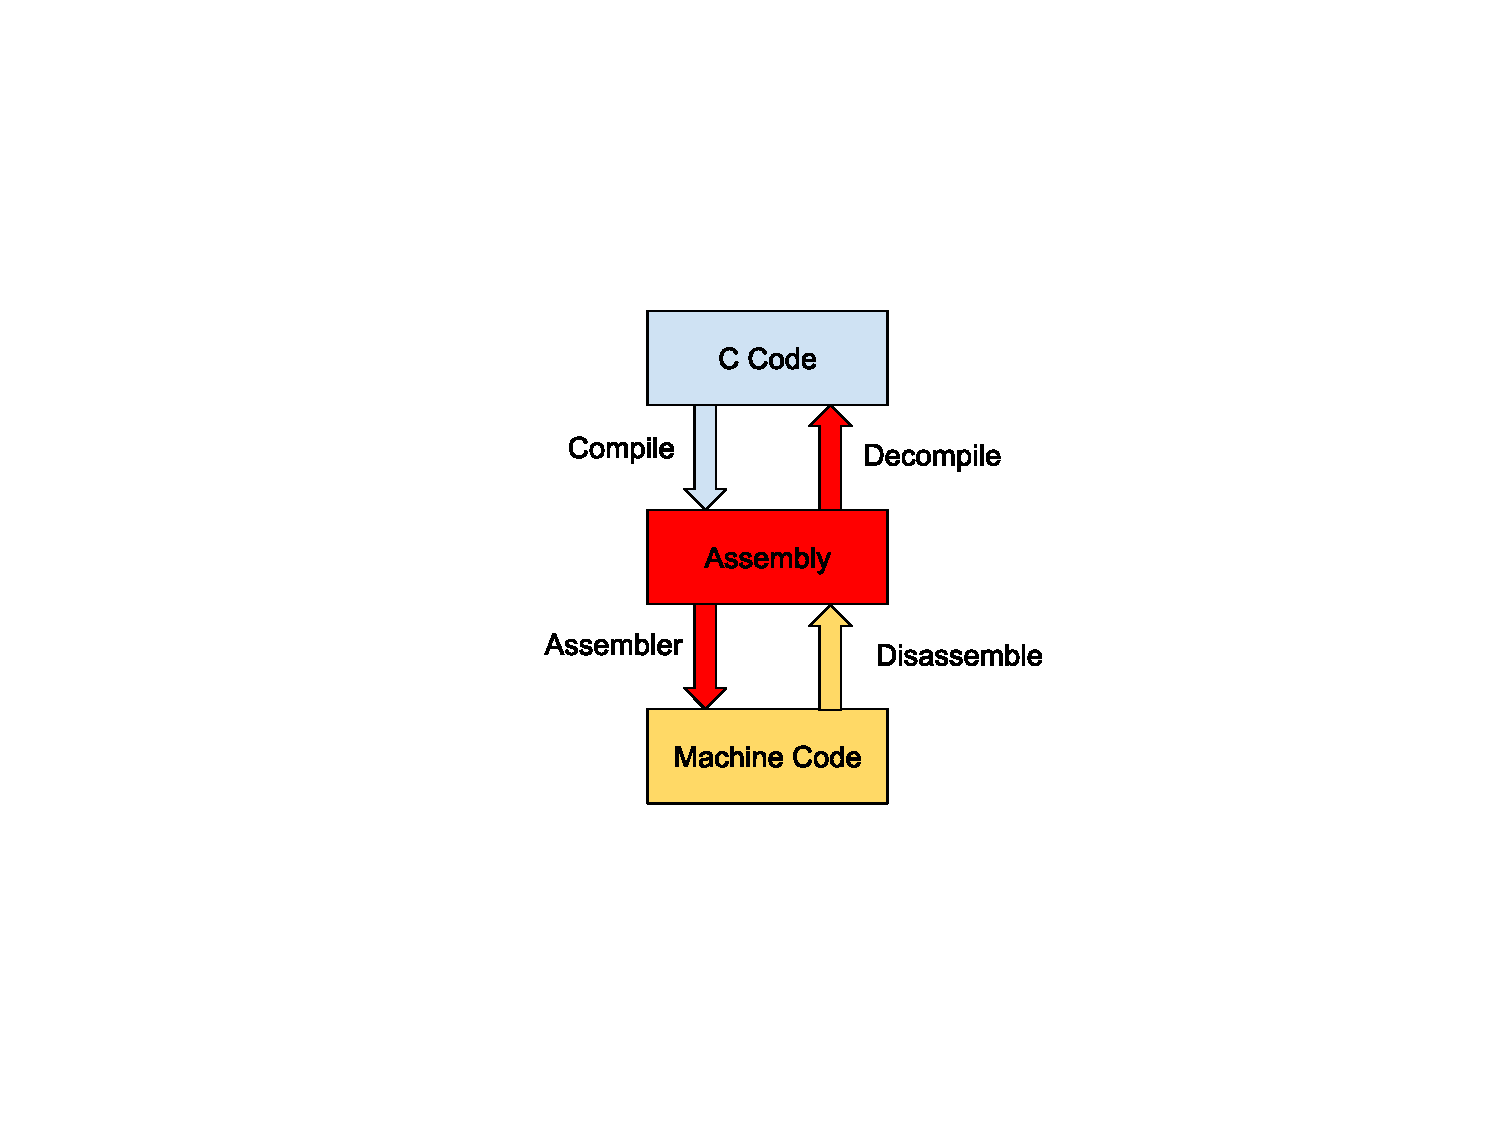
\includegraphics[width=1\textwidth]{images/redocumentation.pdf}
    \caption{Compilation and Decompilation steps \citep{SlideReverse}}
    \label{fig:redocumentation}
\end{figure}
Figure \ref{fig:redocumentation} refers to the case of compiled languages( and we will refers to the them from now on), the image highlight different operations that has to be done in order to go frm the source code to the binary( from top to bottom):
\begin{itemize}
    \item \textbf{Compilation}: from the high level code( say for example C code) you use the compiler \footnote{\url{https://en.wikipedia.org/wiki/Compiler}} to generate a lower level set of instructions, that usually is Assembly code;
    \item \textbf{Assembler}: in this stage you pass from Assembly code, that has an high correspondence with the machine code instructions( it is targeted to a specific architecture \footnote{\url{https://en.wikipedia.org/wiki/Assembly_language}}) into machine code that can be executed.
\end{itemize}
In fact what we usually have is the machine code, the executable file. From it we have to extract useful information to understand what it does, this again requires to revert the previous operations, as shown in \ref{fig:redocumentation}( from bottom to top):
\begin{itemize}
    \item \textbf{Disassemble}: from the machine code of a specific architecture(that can be x86-64 or arm) we get the correspondent Assembly code;
    \item \textbf{Decompile}: from the assembly code we want to obtain a high level code that has generate it, as similar as possible to the original one.
\end{itemize}
The process of generating an executable is not an invertible function \footnote{\url{https://en.wikipedia.org/wiki/Decompiler}} This means that by doing so we loose some information, that makes the inverse process quite harder.
In fact the output of the decompilation stage can vary based on the compiler used to perform compilation, the optimizations enabled( like -O in the gcc compiler) and the presence of metadata present inside of the executable, if for example has been included debug information or if instead it has been stripped of all the metadata.
As previously state some code can also be harder to be decompiled since it has been obfuscated with different techniques, another example is the insertion of instructions that doesn't change the execution flow of instructions, but their insertion broke the alignment and so the decompiler is not able to recognize instructions in the correct way.
The \underline{output of the Disassemble stage} can be analyzed as shown in figure \ref{fig:decompilationoutput}. We can organize block of assembly instructions inside block that are executed sequentially, until some instruction that controls the execution flow are encountered, like jump instructions.
In such cases the flow is divided into different block of other assembly instructions.
\begin{figure}[htp]
    \centering
    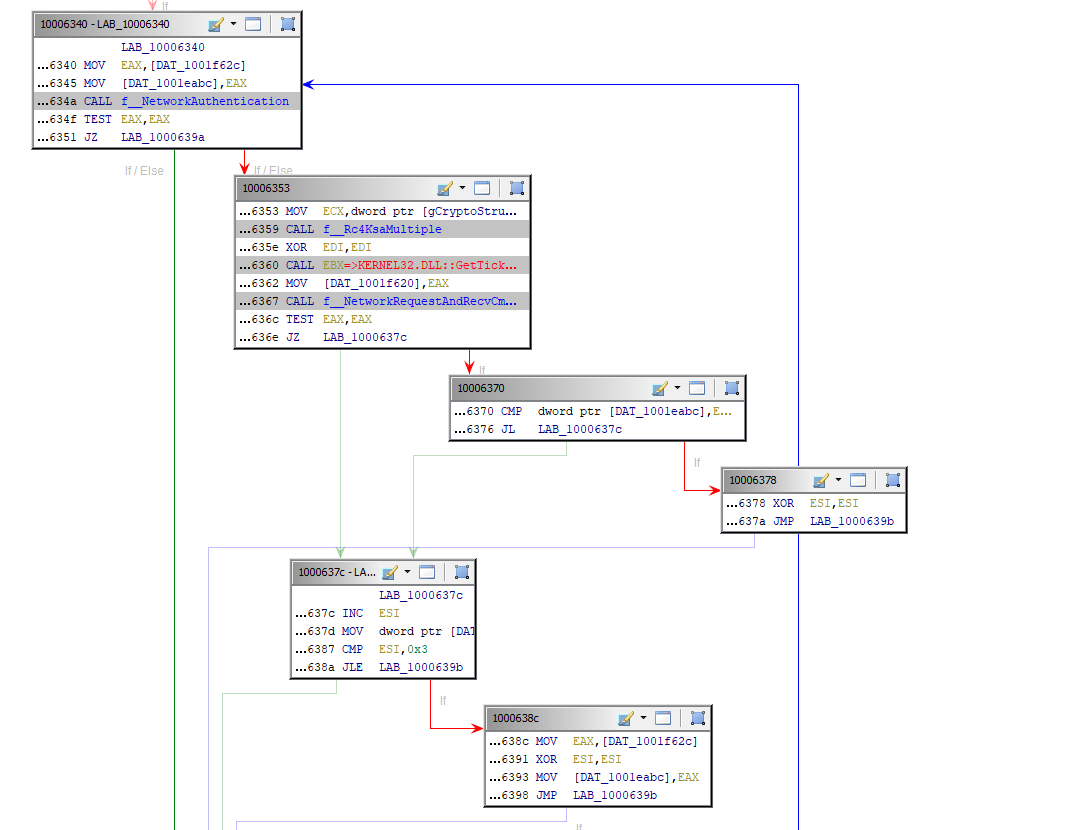
\includegraphics[width=1\textwidth]{images/graphview.png}
    \caption{Analysis of the Decompilation's output stage.}
    \label{fig:decompilationoutput}
\end{figure}
The output of the Decompilation part can be read mode easily since it will be something similar to the original source code that has produced the executable file. 
\begin{figure}[htp]
    \centering
    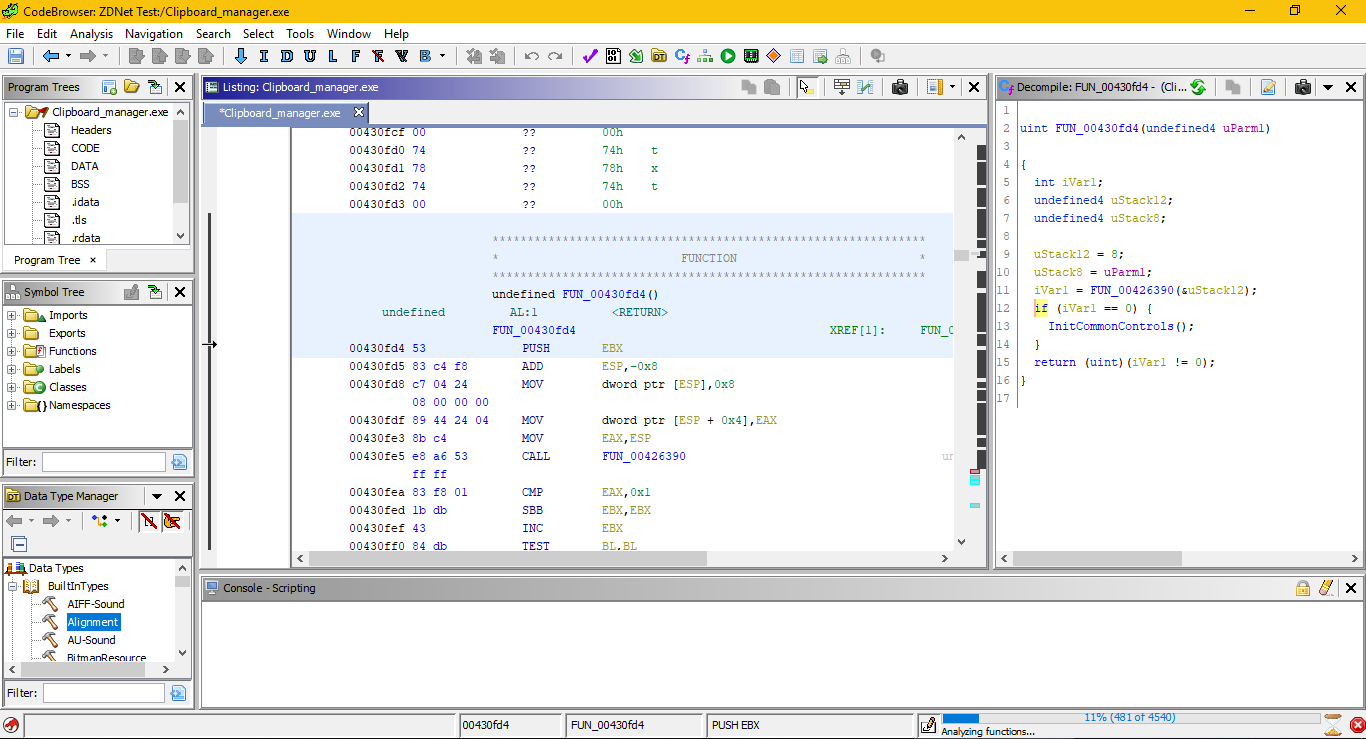
\includegraphics[width=1\textwidth]{images/ghidra.png}
    \caption{Ghidra GUI after analyzing an executable file.}
    \label{fig:ghidraoutput}
\end{figure}
Different tools exists that allows to perform decompilation of an executable. Most famous one are \textit{Ghidra} and \textit{IDA Pro}. Figure \ref{fig:ghidraoutput} show an example output of Ghidra. The reference of supported architecture for decompilation can be found here \footnote{\url{https://en.wikipedia.org/wiki/Ghidra}}.
Ghidra makes use of automated tools that helps in generating the source code starting from the executable. From interface we can look at the whole space of the object file: from the address of the library, to the assembly code, to the constant variables loaded inside the file.
The readability of the output depends on the quality of the tool used to decompile and on the present metadata, but it is more than recommended a user inspection of code, for example to better understand the type of the variable.
\begin{figure}[htp]
    \centering
    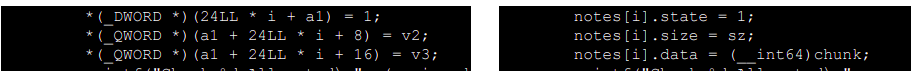
\includegraphics[width=1\textwidth]{images/coderead.png}
    \caption{Code readability after inspection of the struct.}
    \label{fig:coderead}
\end{figure}
As you can see in image \ref{fig:coderead} the code on the right is more readable after inspection if the code, and the definition of a strut hat better fits the memory structure that is used by the executable.
Up to know we have assumed to have under analysis an executable from a \textit{Compiled Language}, but the same things can be applied to \textit{Interpreted Language} \footnote{\url{https://en.wikipedia.org/wiki/Compiled_language}} like for example Java, in which some tool exists in order to analysis the bytecode produced by java \footnote{\url{http://java-decompiler.github.io/}}.
The work done during this stage is important in the first strategy that we will purse in order to discover design features of the programs under analysis: \underline{Static Analysis}.

\clearpage

\subsection{Design Understanding}
The objective of the Reverse Engineering task is to understand the \textit{Design Features} of the program under analysis. So in order to reach this results one can use different techniques, that can be generalized into two main categories: \textbf{Static Analysis} and \textbf{Dynamic Analysis}.

\paragraph{Static Analysis}
What we have seen during the \textit{Redocumentation} stage \ref{section:redocumentation} is what we can think as Static analysis, in fact it is the process of code analysis without regard of its execution or input \citep{LessonReverse}.
From this analysis we can take a look at the:
\begin{itemize}
    \item \textbf{Control flow}: the code is broke down into blocks, that merge together instructions executed sequentially, this separation in block can be done by looking at how the control instructions are placed, like if or while loop \ref{fig:decompilationoutput}, in this way we can try to understand which is the path block executed by the program sequentially, so we can follow the execution flow;
    \item \textbf{Data Flow}: helps in understanding how the data flows inside the program, from the input that we can give to the program to the final outcome of its execution.
\end{itemize}

\paragraph{Dynamic Analysis}
Opposed to Static, Dynamic Analysis rely on the execution of the program regarding on the input provided to it. In this case we try to launch the executable with different inputs and look at the different outcome we got.
\begin{figure}[htp]
    \centering
    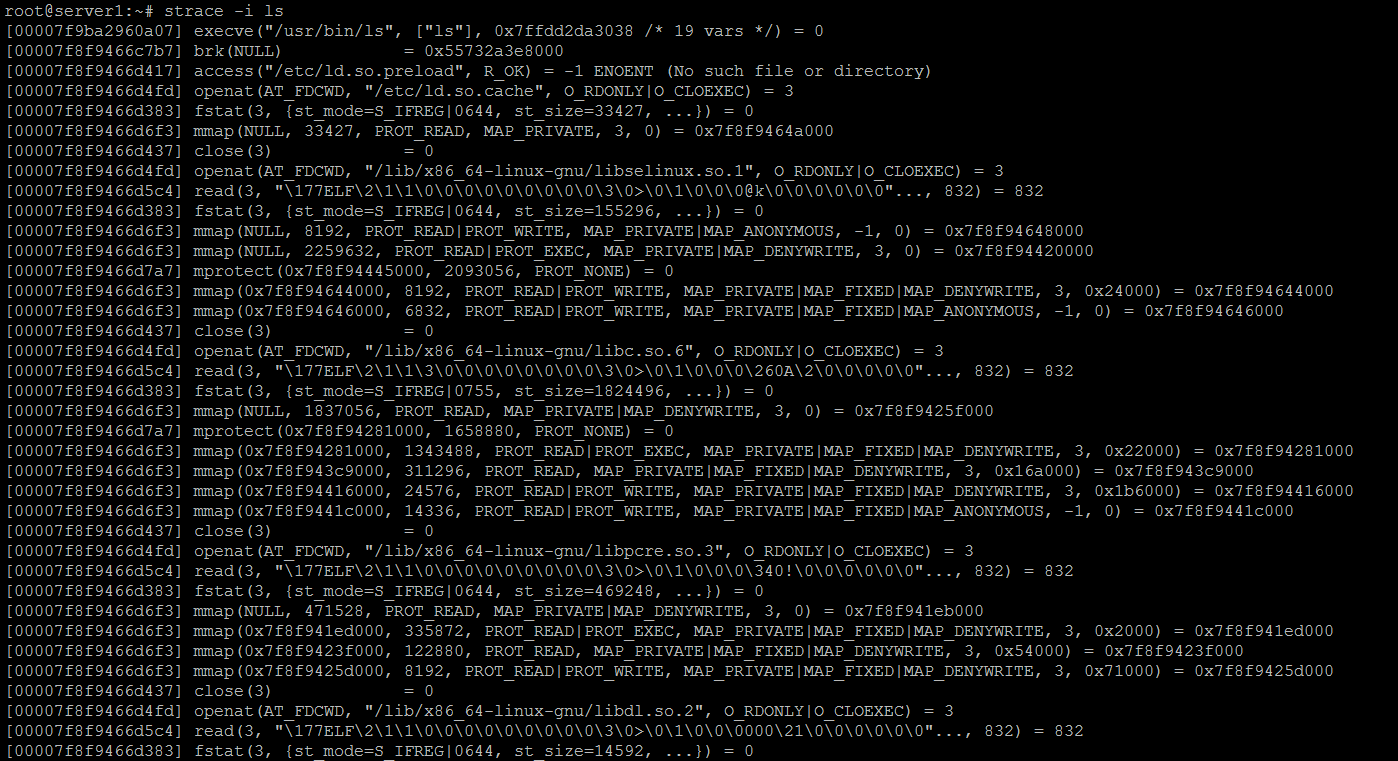
\includegraphics[width=1\textwidth]{images/strace.png}
    \caption{The output of an analysis with strace.}
    \label{fig:strace}
\end{figure}
And by looking at the output returned by the executable we try to guess what the program does. We can also use some other tools to understand what the executable does by looking at the system calls invocation done by it, in this case we can use \textit{strace}\footnote{\url{https://en.wikipedia.org/wiki/Strace}}. As we can see in figure \ref{fig:strace} the output will make a summary of the various system calls done by a certain program.
\textit{Strace} allows to analysis how the executable access to the privileged kernel mode, how the program switch its execution from user mode to kernel mode. Other tools that can be used are \textit{ltrace} and \textit{ptrace}. In general you can look to the access made by the program to the disk memory, to the network usage of the program, etc\dots.
\begin{figure}[htp]
    \centering
    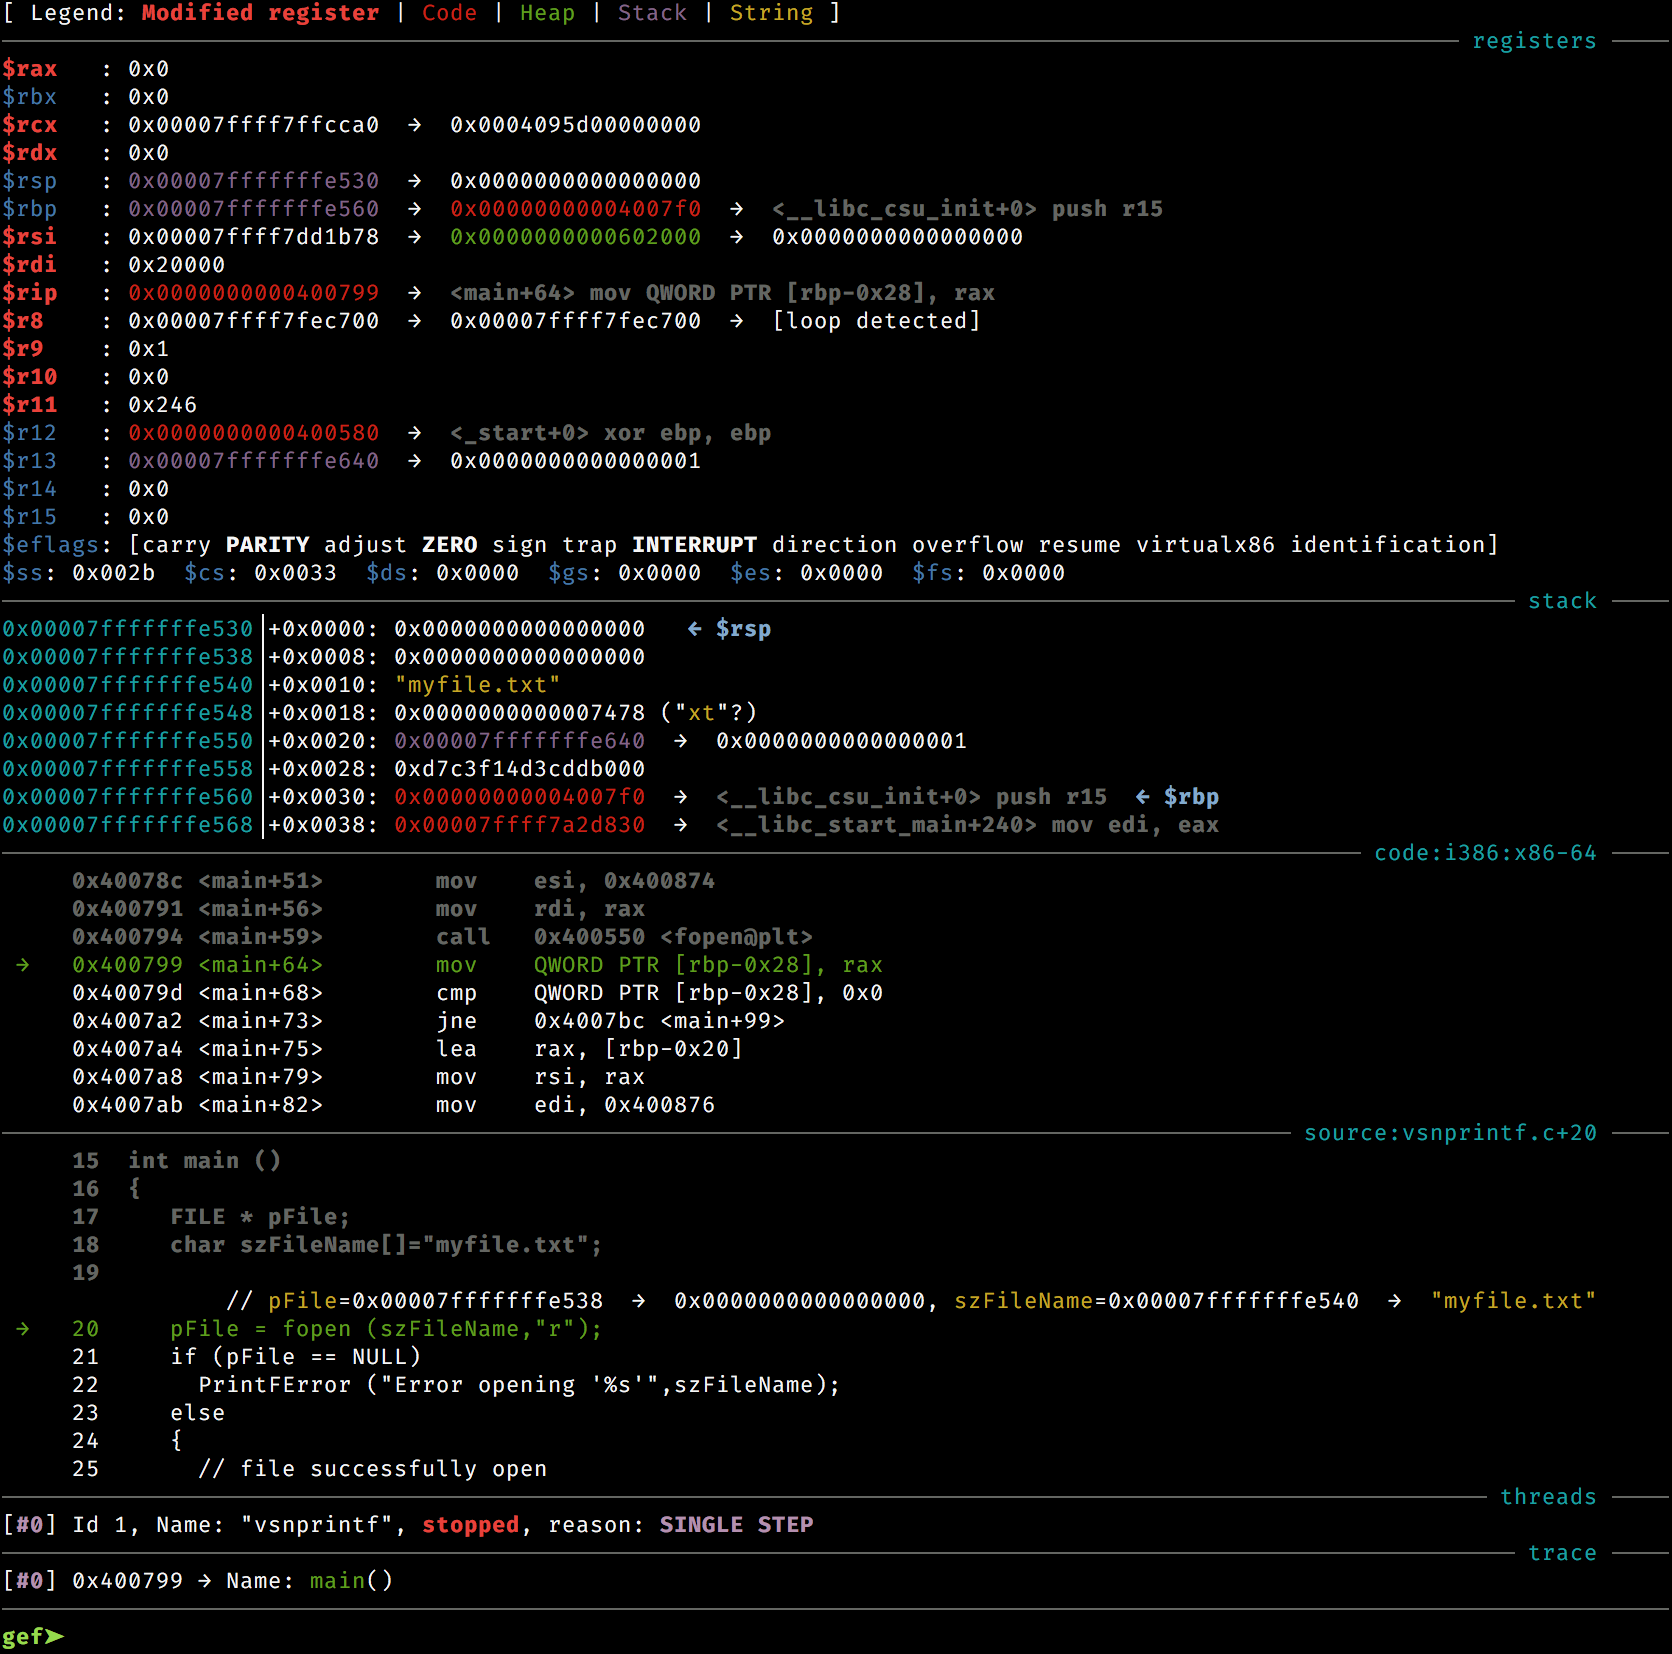
\includegraphics[width=1\textwidth]{images/gdb.png}
    \caption{The output of GDB during a program execution.}
    \label{fig:gdb}
\end{figure}
Since during Dynamic Analysis we have to be able to analyze the behavior of the program as long as it is executing. we can take advantage of another useful tool: the  \textit{Debbuger} It permits to execute an executable in a controlled environment in which we are able to follow the progress of the program\footnote{\url{https://en.wikipedia.org/wiki/Debugger}}. By using breakpoints to stop executions, we can find out the code that is actually executed by the program, and also take a look and modify the content of the registers.
Image \ref{fig:gdb} shows an example of a well known and used debugger: \textit{GDB}. It is quite used debugger that works for different programming languages like C, C++, Pascal, Fortran, etc\dots.
The image shows an example of its usage after hitting a breakpoint: GDB shows the content of the registers and at which line in the assembly code the execution of the program has reached. You can for example use GDB in order to create a dump of the memory that you can better analyze with want we have seen in \ref{section:redocumentation}.
Note that \ref{fig:gdb} shows also to which line of the source code the assembly line corresponds. Obviously this will not be possible in most of the cases when doing Reverse Engineering, since who has made the executable want to make our job harder, so the executable is not shipped with debugging metadata attached to it.

\subsection{Which is the best strategy to adopt?}
\begin{figure}[htp]
    \centering
    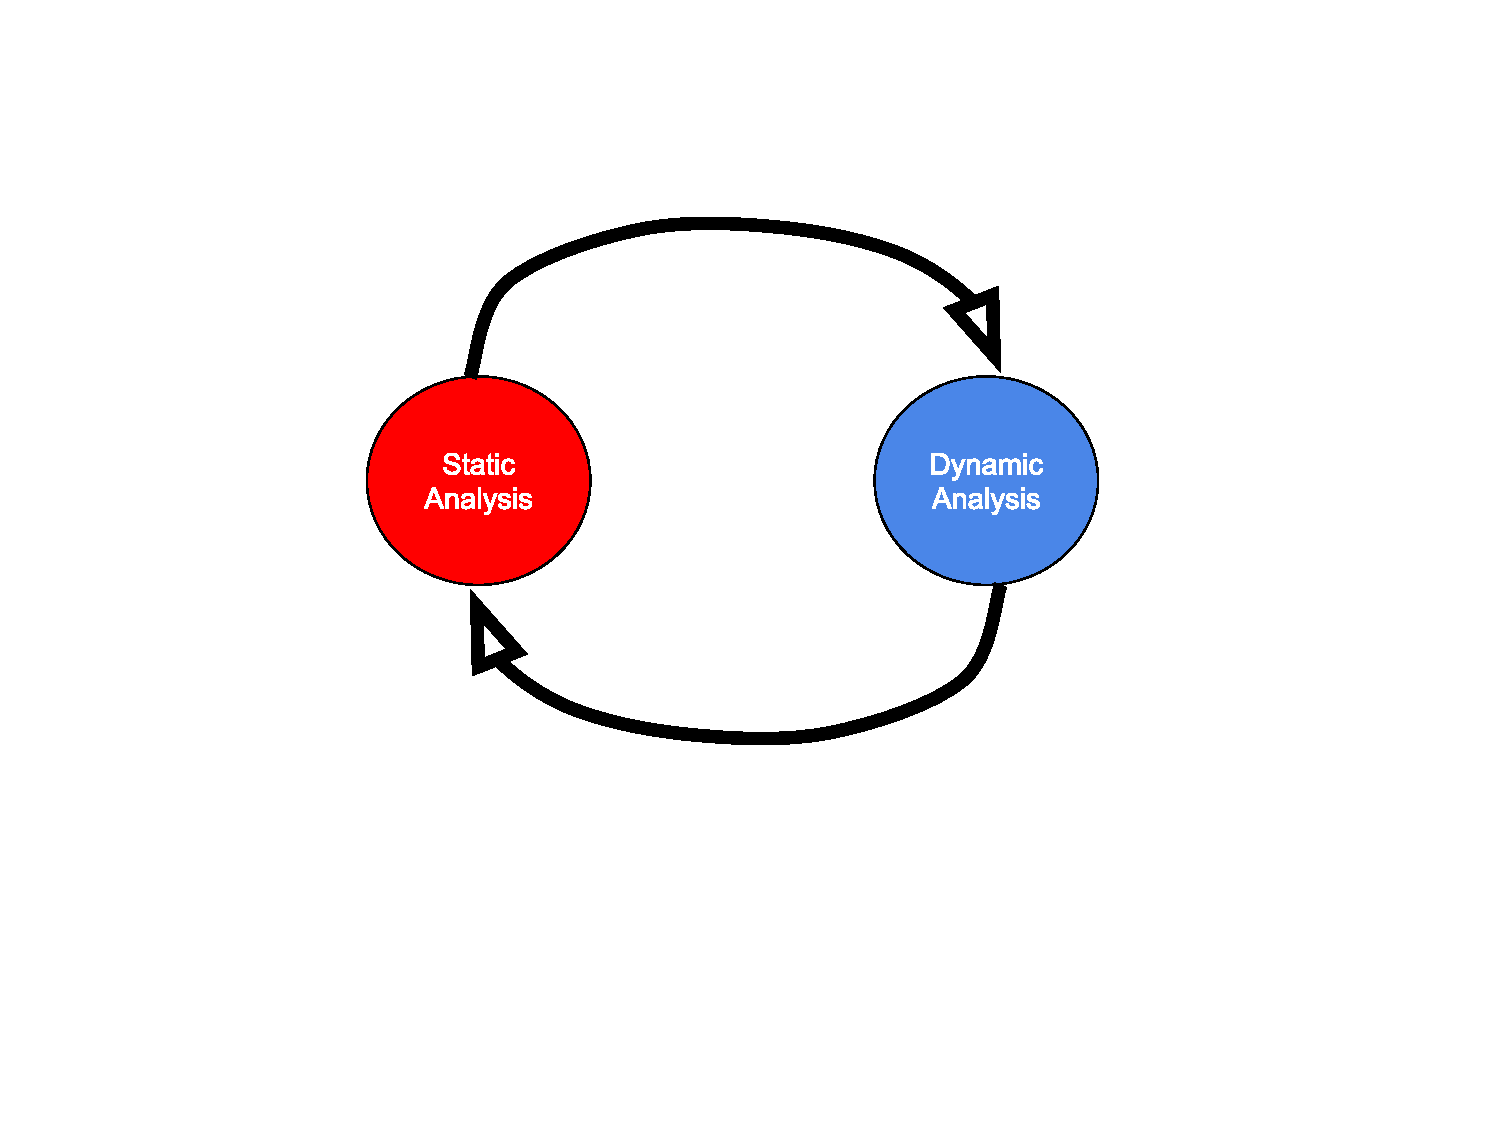
\includegraphics[width=1\textwidth]{images/staticAndDynamic.pdf}
    \caption{Relationship among Static and Dynamic Analysis.}
    \label{fig:gdb}
\end{figure}
One can wonder which approach should choose among the two we have seen so far: if the best idea is to use \textit{Dynamic} or \textit{Static} analysis. Both have disadvantages and advantages: for example static analysis allows to reach an higher code coverage, but if the analyzed software use some obfuscation technique it may be the case that some behaviors are shown only during the execution of the program( is the case of packer\citep{packer}), the go with Dynamic Analysis.
But dynamic analysis has a low code coverage, and so some details in the behavior of a program can be missed.
All of this to highlight that we have to use both approach in synergy: doing static analysis while also doing dynamic analysis, based on the situation we are dealing with. 
So you need to adapt you approach regarding to the software you are approaching to analyze, as we should see in the next example.

\clearpage

\section{keycheck\_baby}
In this section we will cover how to apply the previous theory to a real life scenario, that in this case is the \textit{keycheck\_baby} CTF.
First of all the objective of this CTF is to find the correct flag( a string) as input that is accepted as correct by the executable.
In order to decide which approach we should use we can execute try to analyze the header of the file under analysis with the command as in:
\begin{minted}[linenos, bgcolor=white, escapeinside=!!]{bash}
    $ file keycheck_baby
\end{minted}
In our case as output you will get
\begin{minted}[linenos, bgcolor=white, escapeinside=!!]{bash}
    keycheck_baby: ELF 64-bit LSB shared object, x86-64, version 1 (SYSV), dynamically linked, interpreter /lib64/ld-linux-x86-64.so.2, BuildID[sha1]=7c050cd827cea1dfa736ac05bbac7b343fbf1d01, for GNU/Linux 3.2.0, not stripped
\end{minted}
The important part here is that the executable is \textit{not stripped}\footnote{\url{https://en.wikipedia.org/wiki/Stripped_binary}}, this means that the executable contains also debug information that can be used both by a debugger but it also helps during the decompilation process.
Other important information can be returned by running the following command:
\begin{minted}[linenos, bgcolor=white, escapeinside=!!]{bash}
    $ checksec keycheck_baby
\end{minted}
Which gives as output:
\begin{minted}[linenos, bgcolor=white, escapeinside=!!]{bash}
    Arch:     amd64-64-little
    RELRO:    Partial RELRO
    Stack:    Canary found
    NX:       NX enabled
    PIE:      PIE enabled
\end{minted}
Partial RELRO means that only small parts of the GOT and PLT are writable, while a canary aims in avoiding buffer overflows. NX enabled makes the stack not executable and PIE allows the code to be relocatable in case ASLR is active.
The next step is to start a decompilator to try and analyze the decompiled executable. In our case we will use Ghidra. Ghidra will analyze the executable, and then we can look at the output of the disassemble and decompilation.
First we need to find the entry point of the execution that can be easily found by searching inside the \textit{Symbol Tree} by searching the \textit{main} function, and the output will be as in \ref{fig:keycheckgdb}.
\begin{figure}[htp]
    \centering
    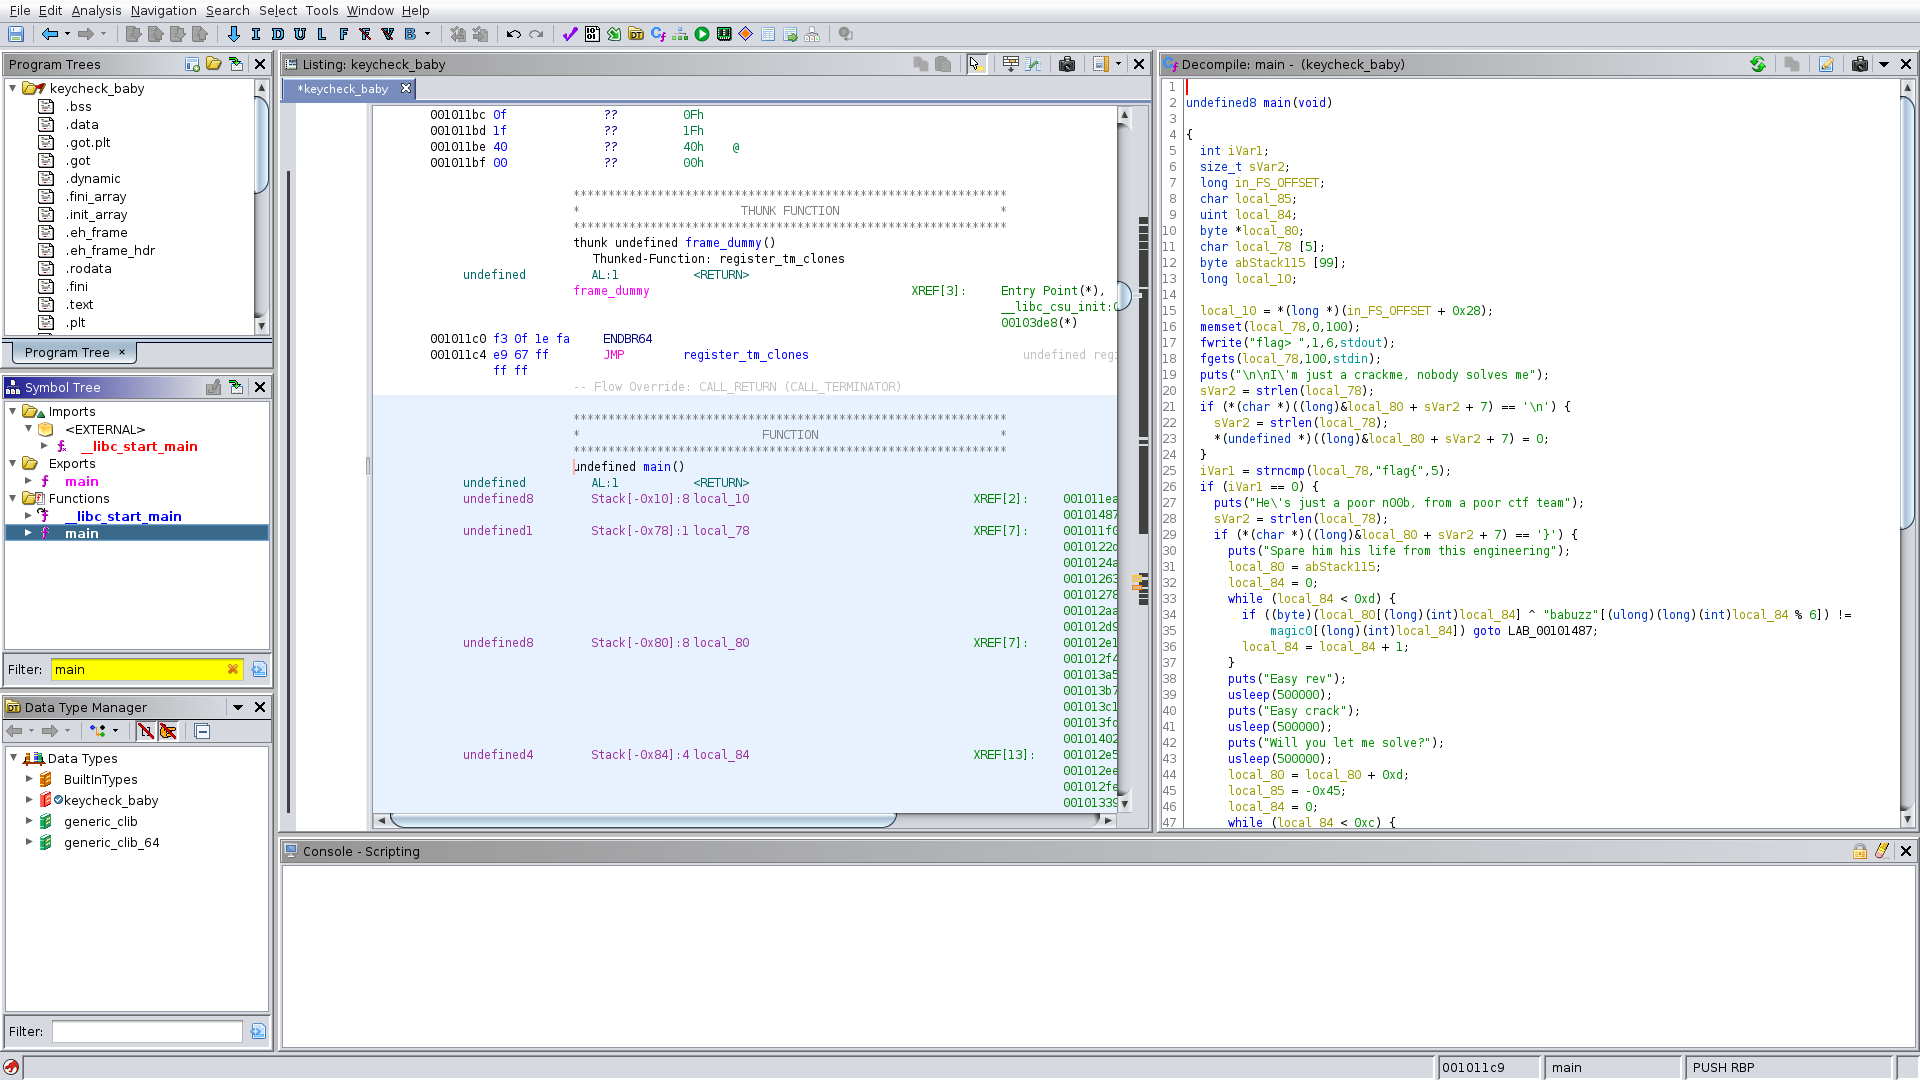
\includegraphics[width=1\textwidth]{images/ghidrakeycheck.png}
    \caption{The output of GDB after analyzing the keycheck executable.}
    \label{fig:keycheckgdb}
\end{figure}
By taking a look a the code we can see that no obfuscation technique has been used since the whole code is there: so we can use as an approach static analysis.
As we have seen in \ref{fig:coderead} in order to make things easier is a good idea to check if we can improve the code readability by retyping variable and assign a different name to them.
For example by saying that the input of the \textit{memset} function is a \textit{char *} in our case.
Now we will take a look at the most important part of the code.
This first part will take as input the flag and it will store it inside the \textit{input} variable. It checks that the string terminate with the string terminator.
At the next step the input is compared with the \textit{flag\{} string:
\begin{minted}[linenos, bgcolor=black, escapeinside=!!]{c}
  iVar1 = strncmp(input,"flag{",5);
  if (iVar1 == 0) {
    puts("He\'s just a poor n00b, from a poor ctf team");
    sVar2 = strlen(input);
    if (*(char *)((long)&input + sVar2) == '}') {
\end{minted}
and it also verifies that the flag ends with a \textit{\}}.
At this point the program checks the first 0xd(13) characters of the input string, by accessing it with the \textit{index}. And it checks that the value of the input string at position index elevated
at the casted int value of the character present in the \textit{babuzz} string at position index \% 6 is the same as the value contained inside the global buffer \textit{maigc0} at position index.
\begin{minted}[linenos, bgcolor=black, escapeinside=!!]{c}
    index = 0;
    while (index < 0xd) {
        if ((byte)(input[(long)(int)index] ^ "babuzz"[(ulong)(long)(int)index % 6]) !=
            magic0[(long)(int)index]) goto LAB_00101487;
        index = index + 1;
    }
\end{minted}
We can find the content of this global buffer from Ghidra, if we double click on it we get the output as in \ref{fig:magic0}.
\begin{figure}[htp]
    \centering
    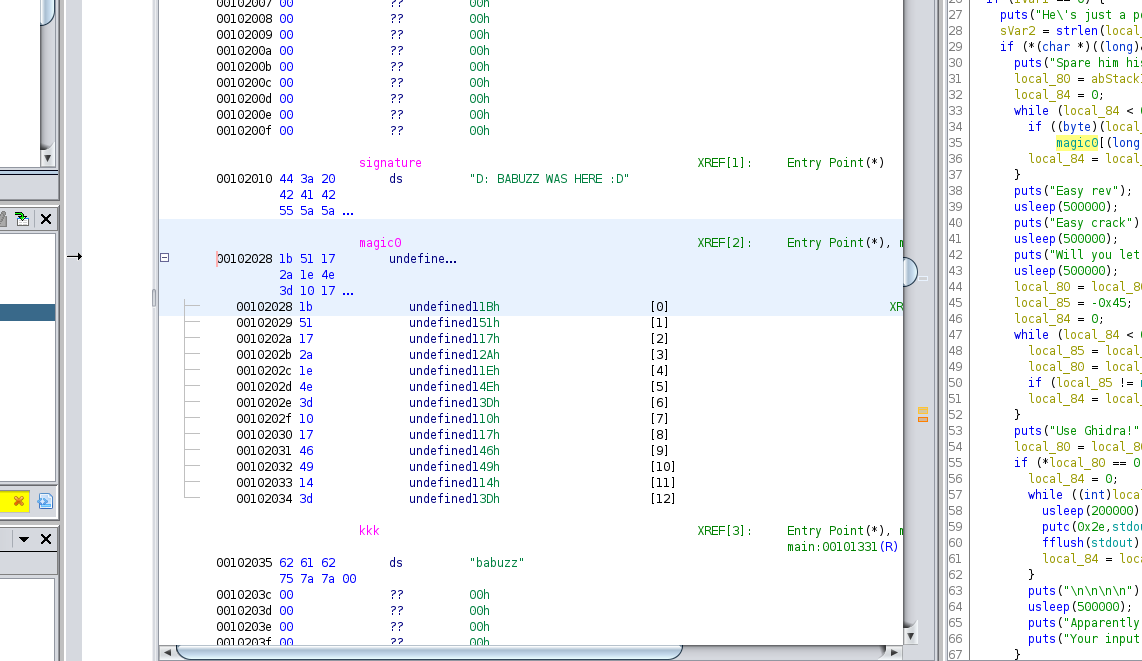
\includegraphics[width=1\textwidth]{images/ghidramagic0.png}
    \caption{The output of GDB after analyzing the keycheck executable.}
    \label{fig:magic0}
\end{figure}
The content of this buffer is represented by the byte stored at each address on the left in the hexadecimal notation.
If this is not the case the flow of execution jumps at the end of the code at the label \textit{LAB\_00101487} before checking the canary, the program exits, so it has not accepted the flag.
\begin{minted}[linenos, bgcolor=black, escapeinside=!!]{c}
    LAB_00101487:
    if (local_10 == *(long *)(in_FS_OFFSET + 0x28)) {
        return 0;
    }
\end{minted}
The next check the executable does is the one in the next snippet of code: first it moves the input forward to the last tested value of it, then it uses a temp value that is initialize to a constant value: 187.
\begin{minted}[linenos, bgcolor=black, escapeinside=!!]{c}
    input = input + 0xd;
    temp = 187;
    index = 0;
    while (index < 0xc) {
        temp = temp + *input;
        input = input + 1;
        if (temp != magic1[(long)(int)index]) goto LAB_00101487;
            index = index + 1;
    }
\end{minted}
At each iteration it compares the content of this temp value and the content of another global buffer \textit{magic1} at the value pointed by the index. Index that is incremented at each iteration until it reaches the value of \textit{0xc}(12).
The value of temp is also updated at each iteration by adding the value contained in the input string at the character that is actually pointed at this iteration, and then used for validation in the check.
Pay attention that the type of temp is \textit{char}, so it must have a value in between 0 and 255, if it goes beyond such value it is casted.
If the execution is able to pass all these checks it finally prints:
\begin{minted}[linenos, bgcolor=black, escapeinside=!!]{c}
    puts("Apparently we let go (:");
    puts("Your input looks like the correct flag \\(^o^)/");
\end{minted}
So if we reach this part of code means that we've got the correct flag.

\subsection{Exploit}
Up to know we have been able in this case to perform only static analysis: with all the information we've obtained with such an analysis we can try to write an exploit that is able to compute the correct flag.
\begin{minted}[linenos, bgcolor=black, escapeinside=!!]{python}
    # Get the content of the two buffer used during the checks
    magic0 = 
        b'\x1b\x51\x17\x2a\x1e\x4e\x3d\x10\x17\x46\x49\x14\x3d'
    magic1 = 
        b'\xeb\x51\xb0\x13\x85\xb9\x1c\x87\xb8\x26\x8d\x07'
    babuzz = "babuzz"

    # Firs part of the flag that is checked
    flag = 'flag{'

    # This is the first check done by the executable
    # It checks the characters in the input string from
    # position len("flag{") to len("flag{")+12 against magic0.
    # And its aim is to find the correct printable character
    # in range between 0 and 256 that pass the checks in the 
    # given input position
    for i in range(0,13):
        for c in range(256):
            # Add the value to the flag string if c
            # elevated at the casted value to
            # int of babuzz string at position i%6
            if int(c) ^ ord(babuzz[i%6]) == magic0[i]:
                flag = flag + chr(c)
                break

    # This is the second check done by the executable
    # It checks the characters in the input string from
    # position len("flag{")+13 to len("flag{")+25 against
    # the content of magic1.
    # As before it checks the condition against all the
    # printable character
    # Start temp with a constant value
    const = 187
    for i in range(0,12):
        for c in range(256):
            # Update the value stored in temp, and cast
            # it to be a char so it needs to have a value
            # between 0 and 256, thus the % operation
            temp = (const + c) % 256
            if temp == magic1[i]:
                const = temp
                flag = flag + chr(c)
                break

    # Add to the obtained flag the closing character
    flag = flag + "}"

    # Finally print the obtained flag
    print(flag)
\end{minted}
This python script has been written by taking advantage of the information we have got during static analysis. It has been written by trying to emulate the behavior of the executable reconstructed after disassembling it.
It assumes that the characters present inside the flag are printable ASCI character, so their int value goes from 0 to 255. The python script replicate the checks done by the executable and tries to find among all the printable characters 
the ones that are able to pass such checks.
So if we run the script we get as output:
\begin{minted}[linenos, bgcolor=white, escapeinside=!!]{bash}
    $ flag{y0u_d4_qu33n_0f_cr4ck1ngz}
\end{minted}
That is the flag accepted by the executable if provided to it as input.


\section{Conclusion}
This document provides an introduction to Reverse Engineering applied to the field of Software Engineering. It illustrates different techniques and approaches used in order to reverse engineering an executable from scratch, by using different tools:
it then applies all of this to a real example taken from a CTF, in which applying the previously introduced tools, providing also a working exploit for it.




\bibliographystyle{plain}
\bibliography{references}
\end{document}
